\chapter{Preliminaries}\label{\positionnumber}
    First we are going to elaborate on the storage-related architecture of databases in general.
    In the following sections we discuss what structures and mechanisms are employed when computing with graph-based data in order to achieve this superior performance.
    There is also a description of the most common traversal schemes and some extensions of these to solve certain classes of problems.
    Finally, at the end of this chapter a specific storage model --- the property graph model --- and a the implementation of this model in a native graph database called Neo4J are described .

\section{Database Architecture}\label{db-arch}
    The reason why we use databases is twofold:
    First, every computer is equipped with different kinds of memory, which differ in size, capacity, speed and price per byte. 
    This induces the so called memory hierarchy, the principle, that few fast, expensive, low capacity memory is used close to the central processing unit, that gets layerwise augmented with inccreasingly slower, less expensive, higher capacity memory. 
    The last layer, which has the highest capacity, defines the overall capacity, while the smallest one is a crucial factor for performance.
    Thus what is shown as secondary storage in \ref{mem-hier} is orders of magnitude slower in terms of both latency and throughput.
    But it is also able to store orders of magnitude more data. 
    \begin{figure}[htp]
        \begin{center}
        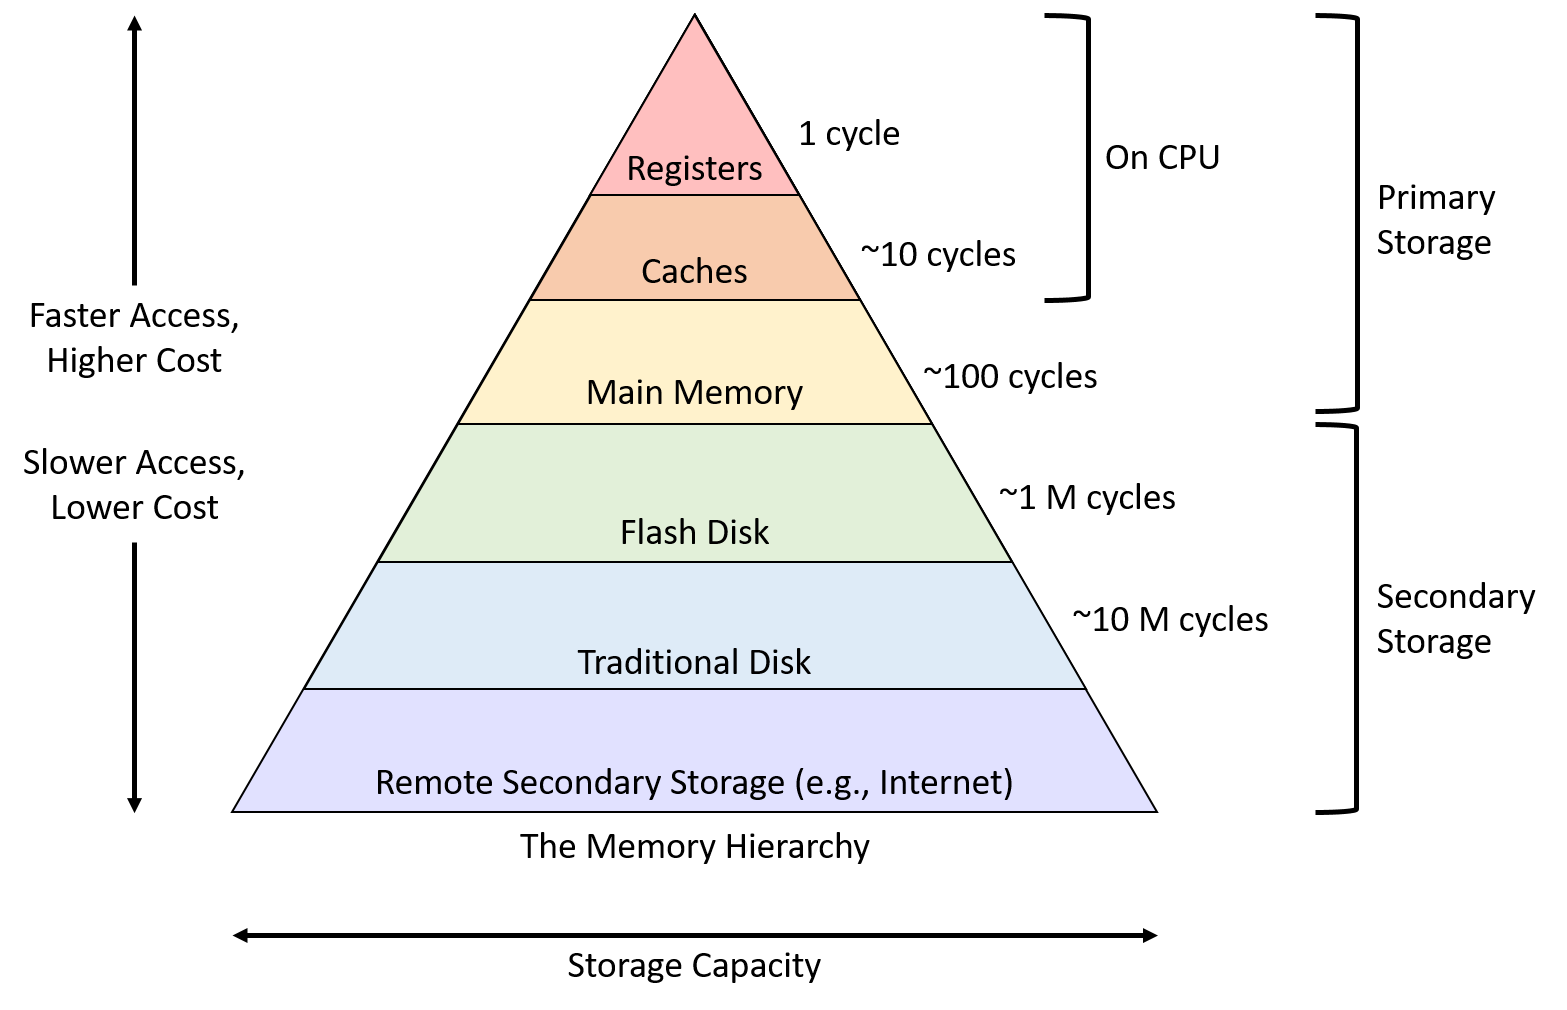
\includegraphics[keepaspectratio,width=0.8\textwidth]{img/03-preliminaries/mem-hierarch.png}
        \end{center}
        \caption{The memory hierarchy used in today's computing systems.} 
        \label{mem-hier}
    \end{figure}
    In order to mitigate the effects of this, the accesses between primary and secondary memory need to be handled very carefully for data intensive --- also called IO bound --- applications.
    Second, the operating system (OS) actually handles the first reason. 
    However application specific payloads enable further optimizations when it comes to how data is stored and accessed.
    Put differently, the operating system is not able to infer certain information, as it does not constrain how data is stored, and as it does not profile in what patterns data is referenced or queried.
    Databases take care of these issues by different mechanisms, which will be lined out from a high level perspective, in order to understand how a database works on its architectural lower levels.
    Put differently, we are not going to discuss query processing, transactions, concurrency related components and recovery facilities.
    Most of the information below is outlined comprehensively in~\autocite{ramakrishnan2000database, silberschatz1997database}
    
    Let us consider the high level architecture of a general database management systems as shown in figure~\ref{dbms_arch} --- with a focus on the storage and access elements.

    \begin{figure}[htp]
    \begin{center}
    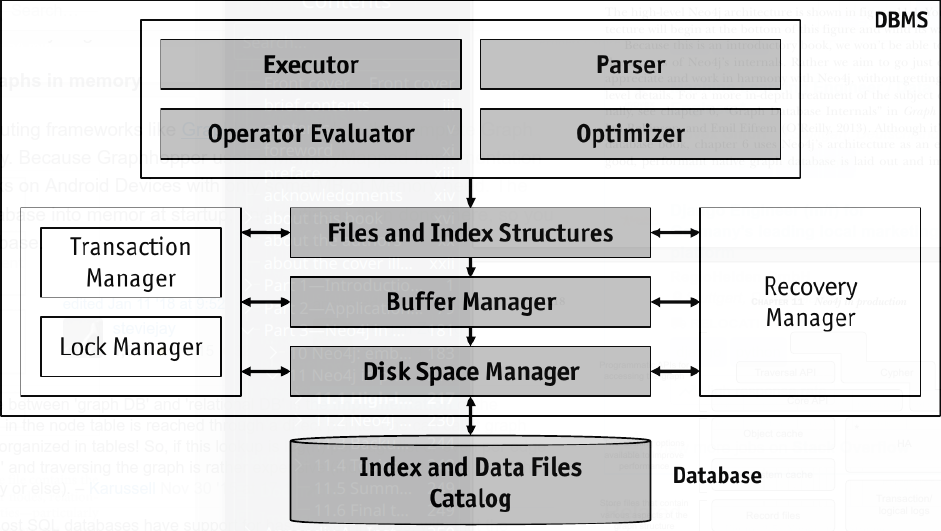
\includegraphics[keepaspectratio,width=.5\textwidth]{img/03-preliminaries/RDBMS.png}
    \end{center}
    \caption{The typical structure of a relational database management system~\autocite{ramakrishnan2000database}.}
    \label{dbms_arch}
    \end{figure}

    The disk space manager, sometimes also called storage manager, handles de-/allocations, reads \& writes and provides the concept of a block: One or many physical disk blocks are grouped to a logical disk block.
    These logical disk blocks are again grouped and brought into main memory (RAM) --- these groups are called a page.
    Optimally both a disk block and a page are of the same size or at least a multiple of each other. 
    Further the database needs to keep track of free blocks in the file: 
    A linked list or a directory must record free blocks and some structure needs to keep track of the free slots either globally or per block. 
    Data locality is a concept that we examine closely in an extra chapter later on.
    To summarize the two most important objectives of a storage manager are to
    \begin{enumerate} 
     \item take care of (de-)allocations of disk space,
     \item abstract storing data on a physical device using the operating system: Files, split into logical disk blocks, accessed using OS facilities, and
     \item provide data structures in order to maintain records within a file, blocks.
    \end{enumerate}
    
    A buffer manager is used to mediate between external storage and main memory. 
    It provides the concept of a page and maintains a designated pre-allocated area of main memory --- called the buffer pool --- to load, cache and evict pages into or from main memory~\autocite{ramakrishnan2000database}.
    A conceptual illustration of this is shown in \ref{buf-man}.
    It's objective is to minimize the number of disk reads to be executed by caching, pre-fetching and the usage of suitable replacement policies. 
    It also needs to take care of allocating a certain fraction of pages to each transaction.

    \begin{figure}[htp]\label{dbms_memory}
        \begin{center}
        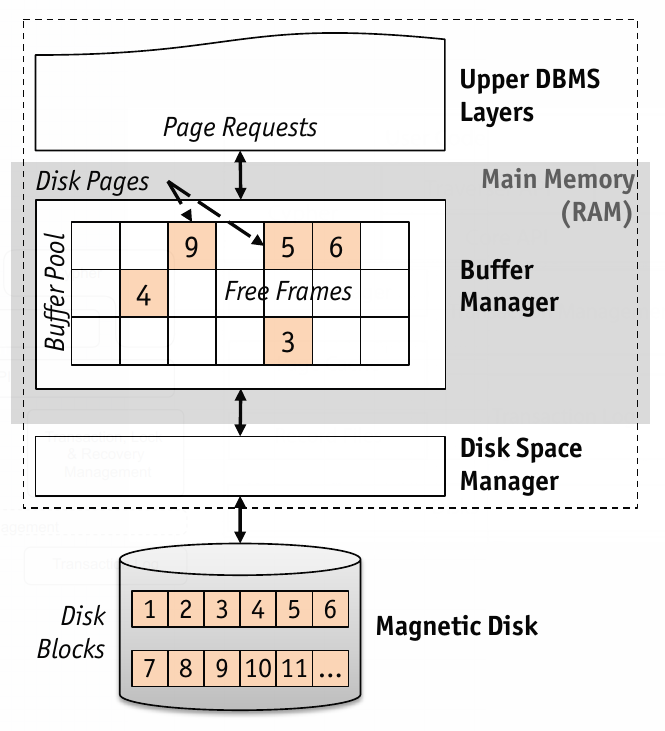
\includegraphics[keepaspectratio,height=0.4\textheight,width=0.5\textwidth]{img/03-preliminaries/RDBMS_memory_view.png}
        \end{center}
        \caption{A visualization of the interaction of a database with memory~\autocite{ramakrishnan2000database}.}
        \label{buf-man}
    \end{figure}

    The final component that is crucial to the storage of data the  of a database management system is the file and record layout, along with possible index structures --- also called the access layer. 
    In order to store data a DBMS may either use one single or multiple files to maintain records. 

    A file consists of a set of blocks split into slots.
    A slot stores one record with each record containing a set of fields.
    Records can be layout in row or column major order.
    That is one can store sequences of tuples or sequences of fields.
    The former is beneficial if a lot of update, insert or delete operations are committed to the database, while the latter optimizes the performance when scans and aggregations are the most typical queries to the system.
    Records may be of fixed or of variable size, depending on the types of their fields. 
    Another option is to store the structure of the records along with pointers to the values of their fields in one files and the actual values in one or multiple separate files. 
    Also distinct types of tables can be stored in different files. 
    For example entities and relations can be stored in different files with references to each other, thus enabling the layout of these two to be specialized to their structure and usage in queries.

    Files may either organize their records in random order (heap file), sorted or using a hash function on one or more fields. 
    All of these approaches have upsides and downsides when it comes to scans, searches, insertions, deletions and updates. 

    To mitigate the effect that result from selecting one file organization or another, one record organization or another, the concept of an index has been introduced. 
    Indexes are auxiliary structures to speed up certain operations or queries that depend on one field. 
    Indexes may be clustered or unclustered. 
    An index over field $F$ is called clustered if the underlying data file is sorted according to the values of $F$. 
    Otherwise the index is called unclustered
    In a similar way indexes can be sparse or dense. 
    A sparse index has less index entries than records, mostly one index entry per block. 
    This can of course only be done for clustered indexes as the sorting of the data file keeps the elements between index keys in order. 
    An index is dense if there is a one to one correspondence between records and index entries. 
    All unclustered indexes are dense indexes.
    There are different variants of storing index entries which have again certain implications on the compactness of the index and the underlying design decisions.
    Finally, there are operators that act upon and use the above structures and mechanisms. 
    Logical operators define an algebraic operation used to process a query.
    Physical operators implement the operation described by logical operators. For each logical operator there may exist multiple different physical implementations using different access methods.

    All these considerations make choosing different file splits, layouts, orderings, addressing schemes, management structures, de-/allocation schemes and indexes a complex set of dependent choices. 
    These depend mainly on the structure of the data to be stored and the queries to be run.
    
\section{Graphs
}\label{\positionnumber}
In this section we first give a definition of graphs as discrete structures and related concepts. Next we introduce and analyze possible data structures and algorithms to represent and operate on graphs. 
        \subsection{Theory}\label{\positionnumber}
            Most of the definitions below follow the notations intorduced in ~\autocite{steger2007diskrete, Gross1998GraphTA, aho1974design, cormen2009introduction, Goodrich2014AlgorithmDA}
        
            A \textbf{graph} $G$ is a tuple $(V, E)$ where $V$ is a non-empty set of vertices (also called nodes). 
            $E$ is a subset of cartesian product of the set vertices $E \subseteq V \times V$, called edges.
            A \textbf{subgraph} is a graph $G' = (V', E')$, where $V' \subseteq V$ and $E' \subseteq E$. 
            
            Two vertices are called \textbf{adjacent}, if there exists an edge between these vertices: 
            \[ u,v \in V \text{ adjacent } \Leftrightarrow \exists e \in E: e = (u, v) \vee e= (v, u).\]
            Given one vertex $v \in V$, the neighbourhood of $v$ are all vertices that are adjacent to $v$: 
            \[N_v = {u \in V | (v, u) \in E \vee (u, v) \in E}.\] 
            A vertex and an edge are called incident, if the edge connects the vertex to another vertex (or itself): 
            \[v \in V, e\in E \text{ incident } \Leftrightarrow \exists u \in V: e = (u,v) \vee (v,u).\]
            The number of neighbours a vertex has is called the \textbf{degree}: 
            \[v \in V: deg(v) = |N_v|.\]
            The average degree of the graph $G$ is defined by:
            \[ \text{deg}(V) = \frac{1}{|V|} \sum_{v \in V}\text{deg}(v)\]
            The set of neighbours connected to a node by incoming edges is called $N_v |_\text{in}$. Analogously we define $N_v |_\text{out}$.             
            One can model villages and roads using a graph. 
            Given two villages that are connected by a road are adjacent. 
            The road and one of the two cities are incident and all villages connected to one specific village by roads are the neighbourhood of this specific village. 
            
            A graph is \textbf{undirected}, if $E$ is a symmetric relation, that is $(u, v) \in E \Rightarrow (v, u) \in E$. 
            Otherwise the graph is called \textbf{directed}, that is the order within the tuple matters and $E$ is not symmetric.             
            Similar to the edges incident to a vertex we can define the incoming and outgoing edges by restricting which of the positions the vertex takes. 
            The set of incoming edges is defined as:
            \[v \in V: \text{In}_v = \{e \in E |u \in V: (u, v) \}.\]
            Similarly the outgoing edges are defined as 
            \[v \in V: \text{Out}_v = \{e \in E |u \in V: (v, u) \}.
            \]
            For example rivers or irrigation systems always have a flow, running exclusively in one direction. 
            This behaviour can be modeled using a directed graph.
            
            Weights can be assigned to both edges and vertices. The graph is called \textbf{weighted}, if either edges or nodes are assigned weights.
            Otherwise it's called unweighted.
            Similarly labels can be assigned to both nodes and edges. 
            In some cases these labels may encode the type of the entity.
            Other arbitrary key-value pairs may be assigned to either the nodes or the edges, the so called properties.           
            An example for a weighted graph is a road network: 
            The vertices are crossings between roads, the roads are the edges and the edge weights represent the distances between the crossings that are connected by the road.
            To include labels, one could distinguish between highways and minor roads or simply assign the name of the road. 
            The former would model the type of the road, while the latter would be an (potentially non-unique) identifier.
            
            In case there may exist multiple edges between the same pair of nodes in the same direction, then the graph is called \textbf{multigraph}. 
            That is, $E_M = (E, M)$ is a multiset, with $M: E \rightarrow \mathbb{N}$. 
            Imagine one tries to model the transportation links between major cities. 
            There are many possible means: Highways, railways, flights and for some sea routes. 
            In particular, two cities may be connected by more than one mean of transportation.
            
            A \textbf{walk} of length $n$ is a sequence of edges, where the target and the source of consecutive edges are equal. Let $u,v,w \in V$. Then a trail is a sequence $(e_i)_{i \in \{0, \dots, n-1\}}$ where $e_i \in E$ and
            \[ \forall j \in \{0, \dots, n-2\}: e_j = (u, v) \Rightarrow e_{j+1} = (v, w)\] 
            A \textbf{trail} is a walk, where all edges are distinct. 
            A \textbf{path} is a trail, where no vertex is visited twice.
            When planning a route from some point to another, one is interested in finding a path between these points.
            More explicitly, one wants to find the shortest possible path. 
            Algorithms to solve this problem setting are given later in this chapter. A \textbf{cycle} is a trail, where the first visited vertex is also the last visited vertex. 
            If you start your route from home, go to work and return home after closing time, your route is a cycle.
            
            A graph is called \textbf{connected}, if for each pair of vertices there exists a path between those: 
            \[G \text{ connected } \Leftrightarrow \forall v_i, v_j \in V: \exists \text{ Path}(u, v).\]
            A \textbf{tree} is a graph, which is connected and cycle-free. 
            A \textbf{spanning tree} is a subgraph $G' = (V', E')$ of $G = (V, E)$, that is a tree and $V' = V$. 
            
            When partitioning a graph, one splits the vertices in disjoint subsets. 
            Thus a \textbf{partition} of a graph is a set of subgraphs $i\in \{0, \dots, n-1\}: G_i = (V_i, E_i)$ of $G$, where 
            \begin{enumerate}
             \item $\forall i,j \in \{0, \dots, n-1\}, i \neq j: V_i \cap V_j = \emptyset$.
             \item $\bigcup_i V_i = V$.
            \end{enumerate}
            
    \subsection{Data Structures}\label{\positionnumber}
        When implementing graphs for computing machinery, there are some possibilities on how to represent the graph in memory.
        We only consider the costs of storing the structure of the graph, for the sake of succintness. 
        Most of the following data structures can be extended to include labels and properties either by using additional fields or pointers. 
        The definitions of the data types and parts of the complexity analysis are based upon~\autocite{Gross1998GraphTA, aho1974design, cormen2009introduction, Goodrich2014AlgorithmDA, steinhaus2010g}. 
        Besides the ones elaborated on below there are the compressed sparse column and row (CSC/CSR) representations, which are used for sparse matrices in arithmetics-heavy applications, like in the library Eigen or Matlab. 
        For more information on these the reader is reffered to~\autocite{steinhaus2010g, Eisenstat1982YaleSM}. In~\ref{data_struct-ex} you can see a visualization of the graph that is used as an example troughout this section.
        
        \begin{figure}[htp]
            \begin{center}
                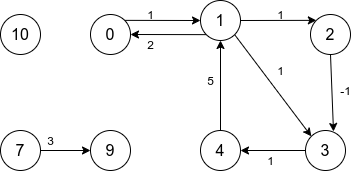
\includegraphics[keepaspectratio,width=0.5\textwidth]{img/03-preliminaries/data_struct_gr.png}
            \end{center}
            \caption{An example graph used throughout this section.} 
            \label{data_struct-ex}
        \end{figure}
        
        \subsubsection*{Unordered Edge List}
        The simplest representation uses an unordered list of edges. 
        That is each element of the data structure carries the information of exactly one edge. 
        For example in a directed, weighted graph, the indices of the source and target node and the weight of the edge are one entry. 
        Additionally an edge list needs to store a list of vertex indices, in order to represent nodes with no edges.
        Overall this results in $\mathcal{|E| + |V|}$ space complexity.
        
        The number of nodes can be retreived in $\mathcal{O}(1)$ assuming that the list data structure stores its size as a filed. 
        The same is true for edges.
        Finding a vertex requires to inspect the list of vertices, thus $\mathcal{O}(|V|)$. 
        Assuming the list stores a pointer to its tail, vertex insertion's asymptotic runtime is $\mathcal{O}(1)$. 
        Deleting a vertex requires a pass over all edges to remove the ones including the particular vertex, in total $\mathcal{O}(|E|)$.
        For edges, the basic operations find, and remove can be executed in linear runtime, i.e. $\mathcal{O}(|E|)$.
        Edge insertion's asymptotic runtime is $\mathcal{O}(1)$, again assuming the list stores a reference to its tail. 
        Deciding wether two vertices are adjacent requires iterating over the list of edges, that is 
        $\mathcal{O}(|E|)$ runtime.
        Finally, finding the neighbourhood $N_v$ of a vertex requires a again a scan of all edges, i.e. an asymptotic runtime of $\mathcal{O}(|E|)$. 
        The same is true for the incoming and outgoing sets of a vertex.
        An example of this data structure is shown in \ref{edgelist}.
        
        \begin{figure}[htp]
         \begin{center}
         \begin{minipage}{0.5\textwidth}
         \begin{minted}[fontsize=\footnotesize]{bash}
          0 1 2 3 4 7 9 10
          \end{minted}
          \begin{minted}{bash}
           0 1 1
           1 0 2
           1 2 1
           2 3 -1
           1 3 1
           3 4 1
           4 1 5
           7 9 3
          \end{minted}
         \end{minipage}%
         \hfill%
         \begin{minipage}{0.5\textwidth}
          \begin{minted}[fontsize=\footnotesize]{bash}
           0 1 1
           1 0 2
           1 2 1
           2 3 -1
           1 3 1
           3 4 1
           4 1 5
           5 6 3
          \end{minted}
         \end{minipage}
         \end{center}
         \caption{%
             An example of the edge list representation of a graph.%
             The left handside uses a list to encode vertex indices, while the right handside assumes consecutive indexes.%
        }
        \label{edgelist}
        \end{figure}

        \subsubsection*{Adjacency Matrix}
        An adjacency matrix of a graph $G$ is a $|V|\times|V|$ matrix where a non-zero entry corresponds to an edge with the weight beeing the value of that entry. 
        Let $A \in |V|\times|V|. u, v \in \{0, \dots, |V| - 1\}$ and $w_{u,v}$ the weight of the edge $e = (u,v) \in E$ then
        \[ a_{uv} = \begin{cases}
                     w_{u,v} & \text{if } (u,v) \in E \\
                     0 & \text{otherwise}
                    \end{cases}
        \]
        Additionally in order to model non-consecutive indices one needs to store a mapping from the actual vertex index to the one used in the matrix --- usually represented by a 2D array. 
        It is also important to note, that adjacency matrix representations are not able to represent multi-graphs without further modification.
        The space complexity of an adjacency matrix is thus $\mathcal{O}(|V|^2 + |V|)$.
                
        The number of nodes can be retreived in $\mathcal{O}(1)$, as it's simply the size of the mapping that is stored.
        For the number of edges, one needs to iterate over all elements of the matrix and count the non-zero entries, which requires one to touch $\mathcal{O}(|V|^2)$ elements.
        Finding a vertex is just an array lookup, thus $\mathcal{O}(1)$.
        Insertion requires to add one row and one column to the matrix, as well as one entry to the mapping. 
        This includes reallocating the matrix which is non-deterministic and independent of the matrix size. But it also requires copying all elements to the new matrix, such that we can estimate the overall asymptotic runtime of $\mathcal{O}(|V|^2)$.
        Deleting a vertex is similar: Either one leaves a gap that may be used on subsequent insertions and simply marks the true id in the mapping as deleted, which would be an $\mathcal{O}(1)$ operation. 
        Alternatively one could imediately reallocate the matrix to free the extra row and column as well as the extra field in the mapping. 
        This would again be non-deteministic, but can again be estimated by copying the elements from the former matrix $\mathcal{O}(|V-1|^2) = \mathcal{O}(|V|^2)$.
        For edges, the basic operations find, insert and remove can be executed in constant runtime, i.e. $\mathcal{O}(1)$, as a simple array access.
        Deciding wether two vertices are adjacent requires just reading what is in the particular array at the index of the two nodes, that is $\mathcal{O}(1)$ runtime.
        Finally, finding the neighbourhood $N_v$ of a vertex requires a again a scan of a row and a column i.e. an asymptotic runtime of $\mathcal{O}(2|V|)$. For the incoming and outgoing sets of a vertex, one needs to access only either a row or a column resulting in $\mathcal{O}(|V|)$ steps per operation.
        An example of this data structure is shown in \ref{adm}.
        
        \begin{figure}[htp]
         \begin{center}
         \begin{minted}[fontsize=\footnotesize]{bash}
            0 1 2 3 4 5 6 7
            0 1 2 3 4 7 9 10
          \end{minted}
          \begin{minted}{bash}
            0 1 0  0 0 0 0 0
            2 0 1  1 0 0 0 0
            0 0 0 -1 0 0 0 0
            0 0 0  0 1 0 0 0
            0 5 0  0 0 0 0 0
            0 0 0  0 0 0 3 0
            0 0 0  0 0 0 0 0
            0 0 0  0 0 0 0 0
          \end{minted}
         \end{center}
         \caption{An example of the adjacency matrix representation of a graph.}
         \label{adm}
        \end{figure}
        
        \subsubsection*{Incidence Matrix}
        An incidence matrix of a graph $G$ is an $|V| \times |E|$ matrix, where each column corresponds to an edge. Each entry in a column is either the positive weight, if the node is the target of the edge or the negative weight, if the node is the source of the edge. Self-loops require a slight extension of this syntax, because here one node would be both source and target such that the entry is zero. One option is to just put the weight as entry of the node.  Another problem is that incidence matrices can not represent negative weights without further extensions.        
        Let $u,v \in \{0, |V|-1\}, j \in \{0, |E|-1\}, A \in |V| \times |E|$ and $a_{v,j}$ the entry at row $v$ and column $j$ of $A$. Let further $w_j$ be the weight of the edge $e_j = (u,v) \in E$. Then 
        \[         a_{vj} = \begin{cases}
                     -w_{v,u} & \text{if } e_j = (v,u) \in E \\
                     w_{u,v} & \text{if } e_j = (u,v) \in E \\
                     0 & \text{otherwise}
                    \end{cases}
        \]
        
        As with adjacency matrices, in order to be able to represent non-consecutive indieces, we need to store a mapping from the true node indices to the ones used in the matrix.
        The space requirements are thus $\mathcal{O}(|V| \cdot |E| + |V|) = \mathcal{O}(|V| \cdot |E|)$.
        
        The number of nodes can be retreived in $\mathcal{O}(1)$, as it's simply the size of the mapping that is stored.
        The number of edges can also be retreived in $\mathcal{O}(1)$ as it's the second dimension of the matrix.
        Finding a vertex is just an array lookup, thus $\mathcal{O}(1)$.
        Insertion requires to add one row and one column to the matrix, as well as one entry to the mapping, as with adjacency lists. 
        Thus the complexity is again the cost of copying the whole matrix $\mathcal{O}(|V| \cdot |E|)$. 
        The same is true for deleting a vertex.         
        In order to find an edge, one needs to scan one row of either the source or the target node of the edge, which requires $\mathcal{O}(|E|)$ steps.
        Insertion and removal of edges correspond to the case of vertices: 
        One would need to reallocate the matrix and copy all elements resulting in an asymptotic runtime complexity of $\mathcal{O}(|V| \cdot |E|)$. 
        Deciding wether two vertices are adjacent requires reading one row and checking for each non-zero element, if the entry in the other nodes row is also non-zero, which has $\mathcal{O}(|E|)$ runtime.        
        Finally, finding the neighbourhood $N_v$ of a vertex requires a again a scan of a row and checking all non-zero entry columns for the neighbour i.e. an asymptotic runtime of $\mathcal{O}(|E|)$. 
        For the incoming and outgoing sets the procedure is almost the same. 
        The difference is, that only positive or negative non-zero columns --- depending on wehter the incoming or outgoing neighbours shall be returned -- have to be checked.
        An example of this data structure is shown in \ref{incm}.
        
        \begin{figure}[htp]
         \begin{center}
         \begin{minted}[fontsize=\footnotesize]{bash}
            0 1 2 3 4 5 6 7
            0 1 2 3 4 7 9 10
          \end{minted}
          \begin{minted}{bash}
            -1  2  0  0    0   0  0
            1  -2 -1 -(-1) 0   5  0
            0   0  1  0    0   0  0
            0   0  0  (-1) 1   0  0
            0   0  0  0    1  -5  0
            0   0  0  0    0   0  0
            0   0  0  0    0   0 -3
            0   0  0  0    0   0  3
          \end{minted}
         \end{center}
         \caption{An example of the incidence matrix representation of a graph.}
         \label{incm}
        \end{figure}
        
        \subsubsection*{Adjacency List}
        In an adjacency list, there is an entry for each vertex in the graph. 
        Each such entry stores the nodes that are adjacent to the vertex, i.e. its neighbourhood $N_v$. 
        It is important to note, that in most implementations only $N_v |_\text{out}$ is the content of the adjacency list.
        When we sum $|N_v |_\text{out}|$ over all vertices of the graph, we count each edge once.
        The space complexity here is $\mathcal{O}(|V| + |V| \cdot \text{deg}(V)) = \mathcal{O}(|V| + |E|)$, as we store each node once and then for each relationship one more node in the corresponding adjacency list containing $N_v |_\text{out}$.

        The number of nodes can be retreived in $\mathcal{O}(1)$, as it's the size of the list.
        For retrieving the number of edges, one needs to iterate over all elements of the node list and sum over their respective adjacency list. This requires $\mathcal{O}(|V| \cdot \text{deg}(V)) = \mathcal{O}(|E|)$ operations.
        Finding a vertex is just a lookup, thus in $\mathcal{O}(1)$.
        Inserting a vertex means simply appending an element to a list which is in $\mathcal{O}(1)$.
        Deleting a vertex requires to iterate over all nodes and their adjacency list in order to remove the occurences as adjacent node and is in $\mathcal{O}(|V| \cdot \text{deg}(V)) = \mathcal{O}(|E|)$.
        Finding an edge, can be done by checking the adjacency list of the source node, and requires to look at $\mathcal{O}(\text{deg}(V))$ elements.
        For the insertion of an edge one needs to append one element to the end of the adjacency list of the source node, which can be done in $\mathcal{O}(1)$.
        Removing an edge again requires to iterate over the adjacency list of the source node and remove the corresponding entry which is again in $\mathcal{O}(\text{deg}(V))$.        
        Deciding wether two vertices are adjacent can be checked by looking at the adjacency lists of two nodes, that is $\mathcal{O}(2 \cdot \text{deg}(V)) = \mathcal{O}(\text{deg}(V))$ runtime.        
        Finally, the outgoing neighbourhood of a vertex, is already stored and can be returned in $\mathcal{O}(1)$.
        In contrast for the incoming neighbourhood one needs to access all vertices' adjacency list and see if the particular vertex is contained in it, resulting in $\mathcal{O}(|V| \cdot \text{deg}(V)) = \mathcal{O}(|E|)$ operations.
        Finding the neighbourhood $N_v$ of a vertex requires to do both of the above queries, that is $\mathcal{O}(|V| \cdot \text{deg}(V) + 1) = \mathcal{O}(|V| \cdot \text{deg}(V))  = \mathcal{O}(|E|)$ operations.  
        Note that in undirected graphs, both directions of all edges exist, i.e. $N_v = N_v |_\text{out} = N_v |_\text{in}$. This means for undirected graphs all neighbourhood queries are in $\mathcal{O}(1)$.      
        An example of this data structure is shown in \ref{adjl}.
        
        \begin{figure}[htp]
         \begin{center}
          \begin{minted}[fontsize=\footnotesize]{bash}
            0 -> (1, 1)
            1 -> (0, 2) -> (2,1) -> (3, 1)
            2 -> (3, -1)
            3 -> (4, 1)
            4 -> (1, 5)
            7 -> (9, 3)
            9
            10
          \end{minted}
         \end{center}
         \caption{An example of the adjacency list representation of a graph.}
         \label{adjl}
        \end{figure}
        
        \subsubsection*{Incidence List}\label{inci}
        This representation is also called incidence table in \autocite{Gross1998GraphTA}.
        The incidence list of a graph $G$ stores for each vertex $v \in V$ the list of edges it is conencted to. 
        The space requirements are thus $\mathcal{O}(|V| + |V| \cdot \text{deg}(V) + |E|) = \mathcal{O}(|V| + |E|)$. 
        In contrast to adjacency lists, incidence lists do not only store the connected vertices but the edges. 
        This comes with an additional cost of $|E|$ memory, but is beneficial when it comes to accessing information. 
        Another benefit is that the additional costs can be mitigated by using references.
        
        Most of the operations have the same complexity class as when using adjacency lists and the same operations are needed. 
        Differences occur first when removing a vertex:
        Instead of having to iterate over all lists and check if the vertex is contained, it is sufficient to look the relevant lists up in the vertexes' list and delete them resulting in $\mathcal{O}(\text{deg}(V))$ operations.        
        Differences also occur, when accessing the neighbourhood. 
        As all edges that are incident to a node are stored, finding all neighbours is an $\mathcal{O}(1)$ operation. 
        Considering the incoming and outgoing neighbourhoods, one only needs to filter the list of incident edges accordingly, which has length $\mathcal{O}(\text{deg}(V))$.
        An example of this data structure is shown in \ref{incidencel}.
        
        \begin{figure}[htp]
         \begin{center}
          \begin{minted}[fontsize=\footnotesize]{bash}
            0 -> (0, 1, 1) -> (1, 0, 2)
            1 -> (1, 0, 2) -> (1, 2, 1) -> (1, 3, 1) -> (4, 1, 5) -> (0, 1, 1)
            2 -> (2, 3, -1) -> (1, 2, 1)
            3 -> (3, 4, 1) -> (1, 3, 1) -> (2, 3, -1)
            4 -> (4, 1, 5)
            7 -> (7, 9, 3)
            9 -> (7, 9, 3)
            10
          \end{minted}
         \end{center}
         \caption{An example of the incidence list representation of a graph.}
         \label{incidencel}
        \end{figure}
        
        
        
        \subsubsection*{Summary}
        While edge lists are able to represent all variations of graphs, the asymptotic runtime for many operations is linear in the number of edges. 
        These are inacceptable costs in many cases.
        
        An adjacency matrix improves the performance for lookups and updates and is thus the standard data structure for many computation heavy tasks and widely used by libraries as Eigen, openBLAS and the Intel math kernel library (MKL)~\autocite{MatrixStorageSchemes-2021-03-05, EigenTheMatrixclass-2020-12-05, MatrixStorageSchemes-1999-10-01}. 
        When dealing with multi-graphs, the adjacency matrix representation requires additional arrays (one per edge ``type``) or is not able to canonically represent them.       
        The incidence matrix is not able to represent self-loops and negative weights without modification, but has some interesting relationships with other matrices. 
        For example, if one multiplies the incidence matrix with its own transpose, one gets the sum of the adjacency matrix and the gradient matrix, i.e. the laplacian matrix~\autocite{brouwer2011spectra}. 
        Further it's useful in physical flow problems and simulations, e.g. when computing the current and resistances in a graph or when simulating micro-circuits~\autocite{weinberg1958kirchhoff}.
        Even tough the incidence matrix requires less space, both options are rather unfeasible when storing large graphs and the incidence matrix provides even worse access times than edge lists.        
        As a side note: The compressed sparse row and compressed sparse column storage formats are very similar to adjacency lists. 
        Insead of using lists, three arrays are used. 
        The first one maps the node to the start index of its relationship in the other two arrays. 
        The other two arrays store the adjacent nodes and the weight of the relationship respectively. 
        CSR/CSC and adjacency lists share most of the algorithmic traits, while requiring least storage. 
        These formats are used for sparse matrix arithmetics in some of the most popular matrix arithmetics libraries, like~\autocite{MatrixStorageSchemes-2021-03-05, EigenTheMatrixclass-2020-12-05, MatrixStorageSchemes-1999-10-01}. 
        
        Finally the adjacency and incidence lists are quite similar in many respects: Both require linear storage space --- which is optimal without further compression. 
        Even tough not optimal for the operations find, insert and remove, both data structures provide access times that are asymptotically better than linear in most cases.
        If the edges are distributed uniformly, we have an average degree of 
        \[ \text{deg}(V) = \frac{2|E|}{|V|} \leq \frac{2 |V|^2}{|V|} = 2 |V| \]
        In real networks, the distribution is often non-uniform but can be modeled using e.g. binomial, poisson or power law type~\autocite{holme2019rare}. 
        A power law distribution would mean that there exist few nodes with a high degree and a lot of nodes with a rather low degree. 
        What is also very applealing is the fact that the adjacency list and especially the incidence list enable one to return the neighbourhood of a vertex in constant or degree-based amount of time. 
        When it comes to traversals of a graph, these are crucial operations as we will see in the next subsection. 
        
        In the table \ref{sumtabds} we summarize the space and runtime complexities of the described data structures and the operations that act upon them. 
        
        \begin{table}
            \begin{tabular}[c]{p{3cm} p{2cm} p{2cm} p{2cm} p{2cm} p{2cm}} \toprule
            & Edge List & Adjacency Matrix & Incidence Matrix & Adjacency List & Incidence List \\ \midrule
            Space Complexity & $\mathcal{O}(|V| + |E|)$ & $\mathcal{O}(|V|^2)$ & $\mathcal{O}(|V| \cdot |E|)$ & $\mathcal{O}(|V| + |E|)$ & $\mathcal{O}(|V| + |E|)$ \\
            Retrieve $|V|$ & $\mathcal{O}(1)$ & $\mathcal{O}(1)$ & $\mathcal{O}(1)$ & $\mathcal{O}(1)$ & $\mathcal{O}(1)$ \\
            Retrieve $|E|$ & $\mathcal{O}(1)$ & $\mathcal{O}(|V|^2)$ & $\mathcal{O}(1)$ & $\mathcal{O}(|E|)$ & $\mathcal{O}(|E|)$ \\
            Find $v \in V$ & $\mathcal{O}(|V|)$ & $\mathcal{O}(1)$ & $\mathcal{O}(1)$ & $\mathcal{O}(1)$ & $\mathcal{O}(1)$ \\
            Insert $v$ to $V$ & $\mathcal{O}(1)$ & $\mathcal{O}(|V|^2)$ & $\mathcal{O}(|V| \cdot |E|)$ & $\mathcal{O}(1)$ & $\mathcal{O}(1)$ \\
            Remove $v$ from $V$ & $\mathcal{O}(|E|)$ & $\mathcal{O}(|V|^2)$ & $\mathcal{O}(|V| \cdot |E|)$ & $\mathcal{O}(|E|)$ & $\mathcal{O}(\text{deg}(V))$ \\
            Find $e \in E$ & $\mathcal{O}(|E|)$ & $\mathcal{O}(1)$ & $\mathcal{O}(|E|)$ & $\mathcal{O}(\text{deg}(V))$ & $\mathcal{O}(\text{deg}(V))$ \\
            Insert $e$ to $E$ & $\mathcal{O}(1)$ & $\mathcal{O}(1)$ & $\mathcal{O}(|V| \cdot |E|)$ & $\mathcal{O}(1)$ & $\mathcal{O}(1)$ \\
            Remove $e$ from $E$ & $\mathcal{O}(|E|)$ & $\mathcal{O}(1)$ & $\mathcal{O}(|V| \cdot |E|)$ & $\mathcal{O}(\text{deg}(V))$ & $\mathcal{O}(\text{deg}(V))$ \\
            $u, v$ adjacent? & $\mathcal{O}(|E|)$ & $\mathcal{O}(1)$ & $\mathcal{O}(|E|)$ & $\mathcal{O}(\text{deg}(V))$ & $\mathcal{O}(\text{deg}(V))$ \\
            $N_v$ & $\mathcal{O}(|E|)$ & $\mathcal{O}(|V|)$ & $\mathcal{O}(|E|)$ & $\mathcal{O}(|E|)$ & $\mathcal{O}(1)$ \\
            $\text{In}_v$ & $\mathcal{O}(|E|)$ & $\mathcal{O}(|V|)$ & $\mathcal{O}(|E|)$ & $\mathcal{O}(|E|)$ & $\mathcal{O}(\text{deg}(V))$ \\
            $\text{Out}_v$ & $\mathcal{O}(|E|)$ & $\mathcal{O}(|V|)$ & $\mathcal{O}(|E|)$ & $\mathcal{O}(1)$ & $\mathcal{O}(\text{deg}(V))$ \\ \bottomrule
         \end{tabular}
         \caption{Space and runtime complexity comparison of the different data types.}
        \label{sumtabds}
        \end{table}

    \newpage
    \subsection{Traversal-based Algorithms}\label{queries}
        \subsubsection*{Random Walk}
            A random walk is a stochastic process, originally defined by Karl Pearson posing the following probelm to the readers or the journal nature in 1905~\autocite{pearson1905problem}: 
            \begin{quote}
                A man starts from a point $O$ and walks $I$ yards in a straight line; he then turns through any angle whatever and walks another $I$ yards in a second straight line. 
                He repeats this process n times. 
                I require the probability that after these $n$ stretches he is at a distance between $r$ and $r + \delta r$ from his starting point, $O$.
            \end{quote}
            The problem has grathered wide interests and has many connections ranging from financial mathematics~\autocite{bachelier1900theorie}, over physics and biology (brownian motion\autocite{brown1828xxvii}) to pure mathematics~\autocite{wiener1976collected}. 
            Random walks are modelled mathematically using markov chains.            
            For further information on the pure mathematical theory the reader is reffered to a comprehensive survey of the topic~\autocite{lovasz1993random}. 
            Our focus will remain database oriented, that is traversal-based.
            In~\autocite{fouss2007random} the authors show, that the generated random walks can be used to compute the similarities of nodes in a graph. 
            This insight is used by a method described in the next chapter.
            
            \begin{algorithm}[htp]
                \KwIn{Graph $G = (V,E)$, number of steps $n$, start vertex id $v\_id$, direction $d$}
                \KwOut{A walk $(e_0, \dots, e_{n-1})$}
                \hrulealg
                \Begin{
                    visited\_edges $\leftarrow$ edge\_t[$n$]\;
                    current\_node\_edges $\leftarrow$ expand($G$, $v\_id$, $d$)\;
                    
                    \For{$i$ from $0$ to $n - 1$}{
                        edge $\leftarrow$ current\_node\_edges[random() $\%$ size(current\_node\_edges)]\;
                        append(visited\_edges, edge)\;
                        current\_node\_edges $\leftarrow$ expand($G$, edge.other\_v\_id, $d$)\;
                    }
                    \Return visited\_edges\;
                }
            \caption{Pseudo-code for a random walk on a graph $G$.}\label{random_walk}
            \end{algorithm}
            
            Pseudo-code describing the algorithm can be found in listing \ref{random_walk}. 
            The code makes two assumptions: The function \mintinline{c}{random()} returns a unsigned integer by drawing from a uniform distribution. 
            The function expand returns the edges with a certain direction of a vertex, given a graph, a vertex (id) and the respective direction.
            
            The runtime complexity of a random walk can be estimated using the number of steps and the average degree of each node in the graph. 
            In each of the $n$ steps we have to construct the list of edges of the currently considered vertex, which has a length of $\mathcal{O}(\text{deg}(V))$. 
            How fast this construction is depends on the data structure that is used. 
            The overall average runtime complexity is $\mathcal{O}(n \cdot \text{deg}(V))$ for incidence lists. 
            For the other data structures, one has to replace the $\text{deg}(V)$ term with the respective runtime of retreiving the neighbourhood of vertex. 
            The average space complexity of a random walk is $\mathcal{O}(\text{deg}(V))$.

        \subsubsection*{Depth First Search}
            One description of the depth first search (DFS) was authored by Charles-Pierre Trémaux in 1818.
            Even though the work was published a lot later, this is the first appearence in modern citation history~\autocite{lucas1891recreations}. 
            He used so called Trémaux trees to solve arbitrary mazes. 
            Each result of a depth first search is such a Trémaux tree.
            These have the property that each two adjacent vertexes are in an ancestor-descendant relationship.
            Even though Trémaux trees themselves are interesting --- for example all Hamiltonian paths are Trémaux trees --- we focus on the description of the depth first search.        
            Depth first search is very similar to backtracking: Chase one path until it proves to be a dead end. 
            Go back to the to the point where you can take a different path, chose that path to chase and reapeat. 
            In fact Donald Knuth considers depth first search and backtracking to be the same algorithm, as both are acting upon a graph. 
            However when backtracking is used, the graph is often implicit~\autocite{Knuth2000DancingL}.        
            Even though DFS is a general traversal schema -- go deep first -- it can also be used for other purposes like finding shortest paths, connected components, testing planarity and many more. 
                    
            \begin{algorithm}[htp]
                \KwIn{Graph $G = (V,E)$, start vertex id v\_id, direction $d$}
                \KwOut{Search numbers DFS, predecessor edges parent}
                \hrulealg
                \Begin{
                    dfs $\leftarrow$ array initialized to $-1$\;
                    parents $\leftarrow$ array initialized to $-1$\;
                    node\_stack $\leftarrow$ create\_stack()\;
                    
                    push(node\_stack, v\_id)\;
                    
                    \While{node\_stack non-empty}{
                        node\_id $\leftarrow$ pop(node\_stack)\;
                        current\_node\_edges $\leftarrow$ expand($G$, v\_id, $d$)\;
                        
                        \For{edge $\in$ current\_node\_egdes}{
                            \If{dfs[edge.other\_v\_id] $= -1$}{
                                dfs[edge.other\_v\_id] $\leftarrow$ dfs[node\_id] + 1\;
                                push(node\_stack, edge.other\_v\_id)\;
                                parent[edge.other\_id] $\leftarrow$ edge.id\;
                            }
                        }
                    }
                    \Return distances, parents\;
                }
            \caption{Pseudo-code for a depth first search on a graph $G$.}\label{dfs}
            \end{algorithm}
            A pseudo-code description of it is given in \ref{dfs}. 
            This version continues its search at the last found edge instead of the last visited edge. 
            This is enable the usage of the implementation for other problems like finding spanning trees, cycles or paths.
            The runtime is again dependent on the data structure, that is used and again the runtime for querying the neighbourhood of a node is the varying term. 
            Each node is visited exactly once and by the handshaking lemma~\autocite{Gross1998GraphTA} it should be clear that we visit each edge twice resulting in an overall worst-case runtime of $\mathcal{O}(|V|+|E|)$. 
            Regarding space complexity, the worst case is that the node stack contains all nodes, i.e. that it is traversed without repetitions or --- put differently --- backtracking. 
            The result is a worst-case space complexity of $\mathcal{O}(|V|)$.
        
        \subsubsection*{Breadth First Search} 
            The first description of beadth first search (BFS) in modern science was given by Konrad Zuse in the course of his Ph.D.thesis on the ''Plankalkühl``. 
            He used it to find connected components~\autocite{zuse1948allgemeinen}. 
            The schema of the breadth first search was also used to find shortest path solutions for mazes and to wire placed electrical components on a printed circuit board (PCB).
            The general traversal scheme in breadth first search is to explore all next neighbours before continuing with those who are more steps away. 
            Thus it first explores one ''level`` exhaustively, before continuing to the next one. 
            In other words: The only difference between DFS and DFS is the data structure that is used: While DFS uses a stack and thus always inspects the element that was inserted last, BFS uses a queue.
            That means it inspects the element that was inserted first.
            An illustrative comparison of DFS and BFS is shown in figure \ref{dfs-bfs}. 
            
            \begin{figure}
            \begin{center}
            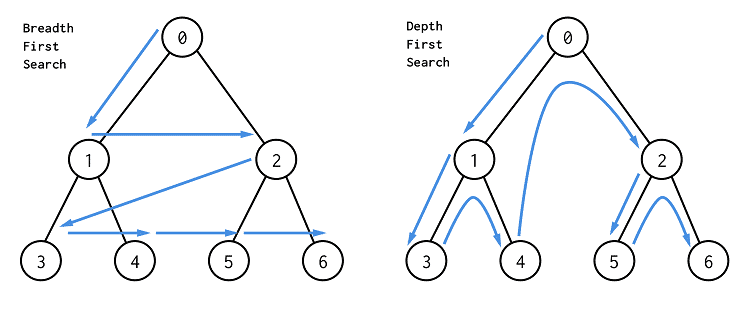
\includegraphics[keepaspectratio,width=0.7\textwidth, height=0.3\textheight]{img/03-preliminaries/bfs-dfs.png}
            \end{center}
            \caption{Comparison between a DFS and a BFS traversal.}\label{dfs-bfs}
            \end{figure}
            
            Like the DFS, the BFS traversal schema can be used to find shortest paths, maximum flows and to test if a graph is bipartite. 
            The space and runtime complexity of the BFS is similar to the complexities of DFS: $\mathcal{O}(|V|)$ space, when all nodes are stored in the queue at the same time. 
            $\mathcal{O}(|V| + |E|)$, since all vertices are visited and each edge is visited twice by the handshake lemma. 
            Pseudo-code for the BFS traversal-scheme is shown in \ref{bfs}. 
            We again make the assumption, that we are using an incidence list as data structure and that the expand operator is implemented accordingly.

            \begin{algorithm}[htp]
                \KwIn{Graph $G = (V,E)$, start vertex id v\_id, direction $d$}
                \KwOut{Search numbers bfs, predecessor edges parent}
                \hrulealg
                \Begin{
                    bfs $\leftarrow$ array initialized to $-1$\;
                    parents $\leftarrow$ array initialized to $-1$\;
                    node\_queue $\leftarrow$ create\_queue()\;
                    
                    enqueue(node\_queue, v\_id)\;
                    
                    \While{node\_queue non-empty}{
                        node\_id $\leftarrow$ dequeue(node\_queue)\;
                        current\_node\_edges $\leftarrow$ expand($G$, v\_id, $d$)\;
                        
                        \For{edge $\in$ current\_node\_egdes}{
                            \If{bfs[edge.other\_v\_id] $= -1$}{
                                bfs[edge.other\_v\_id] $\leftarrow$ bfs[node\_id] + 1\;
                                enqueue(node\_queue, edge.other\_v\_id)\;
                                parent[edge.other\_id] $\leftarrow$ edge.id\;
                            }
                        }
                    }
                    \Return distances, parents\;
                }
            \caption{Pseudo-code for a breadth first search on a graph $G$.}\label{bfs}
            \end{algorithm}
        
            \subsubsection*{Dijkstra} In the original formulation, Edsger Dijkstra formulated the algorithm as a solution to the problem of finding a shortest path between two nodes~\autocite{dijkstra1959note}. 
            Many variants and extensions exist of which we are going to discuss two: A$^*$ and ALT~\autocite{hart1968formal, goldberg2005computing}. 
            One slight variation makes it possible to find all shortest path from a given source node.
            The algorithm however imposes a restriction on the graph.
            Only positive weights are allowed as otherwise a negative cycle results in an infinite loop~\autocite{cormen2009introduction}. 
            
            Conceptually Dijkstra's algorithm assigns each node in the graph a distance. 
            The source node has the distance 0, while all other vertices have a distance of infinity at the beginning.
            Then it gradually considers the next ''shortest`` edge to take.
            That is the distance of the already taken path to a certain node (at the beginning it's zero) is added to an edge weight such that the sum of both is minimal. 
            In order to efficiently compute the minimum a priority queue or a fibonacci heap is used to define the traversal order. 
            An array stores the distances from the source to the already visited nodes, while the queue is filled with their neighbours along with the distance to them (i.e. the path to the predecessor plus the weight of the edge to be taken). 
            The vertex with the shortest total distance is visited until all vertices are visited or the target vertex is reached.
            
            Pseudo code for the variant that computes all shortest paths can be found in \ref{dijkstra}. 
            The runtime complexity of Dijkstra's algorithm is $\mathcal{O}(|E| \cdot T_d + |V| \cdot T_m)$ where $T_d, T_m$ stand for the complexities to update the distance of a path and to extract the minimum.
            Besides the new neccissity to select the element to inspect based on priorities and to maintain those, the runtime complexity is equivalent to what we had with BFS.        
            We use a min-priority queue here, which is simpler to implement but yields a sub-optimal runtime: 
            $T_d, T_m \in \mathcal{\log(|V|)}$. 
            Overall the asymptotic runtime complexity using a min-priority queue is $\mathcal{O}((|V| + |E|)\log(|V|))$~\autocite{Goodrich2014AlgorithmDA}.        
            One can also use plain arrays, which requires a minimum search and no update of the priority. 
            The minimum search is linear, i.e. $\mathcal{O}(|V|)$ and priorities can be updated in $\mathcal{O}(1)$. 
            Overall we have $\mathcal{O}(|E| + |V|^2)$~\autocite{Goodrich2014AlgorithmDA}.        
            Finally more advanced data structures can be used, like a Fibonacci-Heap~\autocite{cormen2009introduction}. 
            These make it possible to update the priority in $\mathcal{O}(1)$ and still find the minimum in $\mathcal{\log(|V|)}$. 
            This yields the optimal asymptotical runtime of $\mathcal{O}(|E| + |V|\log(|V|))$. 
            The worst case space complexity is again $\mathcal{O}(|V|)$, that is when all nodes are stored in the queue at the same time. 
            As there is only one shortest path (paths of equal size are discarded) to each node, the queue contains each node only once.
            
            \begin{algorithm}[htp]
                \KwIn{Graph $G = (V,E)$, source vertex id v\_id, direction $d$}
                \KwOut{Path distance distances, predecessor edges parent}
                \hrulealg
                \Begin{
                    distances $\leftarrow$ array initialized to $\infty$\;
                    parents $\leftarrow$ array initialized to $-1$\;
                    path\_queue $\leftarrow$ create\_min\_prio\_queue()\;
                    
                    enqueue(path\_queue, v\_id)\;
                    
                    \While{path\_queue non-empty}{
                        node\_id $\leftarrow$ dequeue(path\_queue)\;
                        current\_node\_edges $\leftarrow$ expand($G$, v\_id, $d$)\;
                        
                        \For{edge $\in$ current\_node\_egdes}{
                            \If{distances[edge.other\_v\_id] $\geq$ distances[node\_id] + edge.weight}{
                                distances[edge.other\_v\_id] $\leftarrow$ distances[node\_id] + edge.weight\;
                                enqueue(path\_queue, edge.other\_v\_id)\;
                                parent[edge.other\_id] $\leftarrow$ edge.id\;
                            }
                        }
                    }
                    \Return distances, parents\;
                }
            \caption{Pseudo-code of the Dijkstra's algorithm for finding shortest paths from a node $v$ to all other nodes in a graph $G$.}\label{dijkstra}
            \end{algorithm}
        
        
        \subsubsection*{A*}
            The A$^*$ was originally invented in the late 60's to be used for path planning of a robot. 
            It's an extension of Dijkstra's algorithm, that does not just use the distance as metric of priority, but adds a heuristic $h: V \rightarrow \mathbb{R}$ to the distance: 
            $v \in V: f(v) = \text{distance}(v) + h(v)$, that has to fulfill certain conditions:
            With $u,v \in V$ and $\min\text{ distance}(u)$ the minimal distance from the  vertex $u$ to the goal vertex
            \[ \forall u,v: h(u) \leq d(u, v) + h(v) \wedge h(u) \leq \min\text{ distance}(u).
            \]
            The former condition is called consistency, the latter admissibility. 
            As all consistent heuristics are admissible the first condition is sufficient.
            An example for graphs with an euclidean coordinate system is the euclidean distance~\autocite{hart1968formal}.
            
            \ref{a-star} shows pseudo code for the algorithm. The runtime is of course dependent on the complexity of the heuristics.
            Overall we have the same worst case complexity as with Dijkstra's algorithm for the constant heuristic: 
            $\forall v \in V: h(v) = 0$. 
            The best case of the A$^*$ algorithm is when the heuristic is equal to the distance from the current vertex to the goal vertex. 
            Then exactly $\min \text{distance}$ nodes are visited and the algorithm is in $\mathcal{O})\min \text{distance})$, which is the global optimum for a single source shortest path problem.
            
            \begin{algorithm}[htp]
                \KwIn{Graph $G = (V,E)$, heuristic $h$, source vertex id v\_source, target node v\_target, direction $d$}
                \KwOut{Path p}
                \hrulealg
                \Begin{
                    parents $\leftarrow$ array initialized to $-1$\;
                    path\_queue $\leftarrow$ create\_min\_prio\_queue()\;
                    
                    enqueue(path\_queue, v\_id)\;
                    
                    \While{path\_queue non-empty}{
                        node\_id $\leftarrow$ dequeue(path\_queue)\;
                        
                        \If{node\_id = v\_target}{
                            \Return construct\_path(parents)\;
                        }
                        
                        current\_node\_edges $\leftarrow$ expand($G$, v\_id, $d$)\;
                        
                        \For{edge $\in$ current\_node\_egdes}{
                            \If{distances[edge.other\_v\_id] $\geq$ distances[node\_id] + edge.weight + $h($edge.other\_v\_id)}{
                                distances[edge.other\_v\_id] $\leftarrow$ distances[node\_id] + edge.weight + $h($edge.other\_v\_id$)$\;
                                enqueue(path\_queue, edge.other\_v\_id)\;
                                parent[edge.other\_id] $\leftarrow$ edge.id\;
                            }
                        }
                    }
                    \Return empty\_path()\;
                }
            \caption{Pseudo-code of the A$^*$ algorithm for finding shortest paths from a node $v$ to a node $u$ in a graph $G$.}\label{a-star}
            \end{algorithm}
            
        \subsubsection*{ALT}
            ALT stands for A$^*$, landmarks, triangular inequality. 
            It is an extension of A$^*$ which uses landmarks and the triangular inequality as a heuristic. 
            A landmark is a vertex $v \in V$, which is used for orientation. 
            With ALT we select a set of landmarks $L$ and execute Dijkstra's algorithm on each of those, such that we have a set of distances per node and landmark.
            More explictly we use that $d(L_i, v) - d(L_i, w) \leq d(v,w)$ as a lower bound to the actual distance.
            
            In the first step --- the preprocessing step --- of ALT we compute and store these values, giving a space overhead of $\mathcal{O}(|L| \cdot |V|)$. 
            This is shown as pseudo code in \ref{alt-pre}.
            In the second step --- the actual query --- for every node we check which landmark gives the best lower bound of the actual distance.
            This is done by maximizing the following term per node and using it as heuristic $h$.
            With $v_t$ beeing the target node: 
            \[ h(v) = \max_i d(L_i, v) - d(L_i, v_t) \]
            After that A$^*$ is executed as described in \ref{alt-query}.
            
            Besides the additional space that is used we also execute Dijkstra's algorithm $|L|$ times and have an asymptotic complexity of $\mathcal{O}(|L| \cdot (|E| + |V| \log |V|))$ using an incidence list to store the graph and a Fibonacci heap as data structure for the priority queue. 
            Regarding space we need $\mathcal{O}(|V| \cdot (1 + |L|))$. 
            For small values of $|L|$ we preserve the worst case complexity as average case complexity of ALT.
            What we gain by that is that the precomputations take the main runtime penalty while providing a reasonably good heuristic depending on the selection of the landmarks~\autocite{goldberg2005computing}. 
            How to select the landmarks is discussed in~\autocite{Goldberg2005ComputingPS}.
            
            
            \begin{algorithm}[htp]
                \KwIn{Graph $G = (V,E)$, direction $d$, number of landmarks $nl$}
                \KwOut{Precomputed distance from each landmark to all other vertices $\text{landmarks}[|L|][|V|]$}
                \hrulealg
                \Begin{
                    \tcc{Preprocessing stage.}
                    \tcc{Done in advance and only once.}
                    $L \leftarrow$ select\_landmarks($G$, $nl$, $d$)\;
                    \For {$l_i \in L$}{
                        \For{$v_j \in V$}{
                            landmark$[i] = \text{dijkstra}(G, l_i, d)$.distances\;
                        }
                    }
                    \Return landmarks\;
                }
            \caption{Pseudo-code of the preprocessing stage of ALT.}\label{alt-pre}
            \end{algorithm}
            \begin{algorithm}[htp]
                \KwIn{Graph $G = (V,E)$, source vertex id v\_source, target node v\_target, direction $d$, $\text{landmarks}[|L|][|V|]$}
                \KwOut{Path p}
                \hrulealg
                \Begin{
                    \tcc{Query stage.}
                    \tcc{Done for every shortest path query.}
                    \For{$v \in V \setminus \{v_t\}$}{
                        $h[v] \leftarrow \max_i$ landmarks[i][v]$ - $landmarks[i][v\_target] 
                    }
                    \Return a-star($G, h$ v\_source, v\_target, $d$)\;
                }
            \caption{Pseudo-code of the query stage of the ALT algorithm for finding shortest paths from a node $v$ to a node $u$ in a graph $G$.}\label{alt-query}
            \end{algorithm}

\section{Graph Databases}
    Relational databases store data in tables.
    The links considered in this category of DBMS are mostly used to stitch together the fields of a record stored in different tables into one row again, after it has been split to satisfy a certain normal form.
    Of course one may also store tables where one table stores nodes and the other table's fields are node IDs to represent relationships.

    However, in order to traverse the graph, one has either to do a lot of rather expensive look ups or store auxiliary structures to speed up the look up process.
    In particular when using B-trees as index structure, each look up takes $\mathcal{O}(\log(n))$ steps to locate a specific edge.
    Alternatively one could store an additional table that holds incidence lists such that the look up of outgoing or incomming edges is only $\mathcal{O}(\log(n))$ which would speed up breadth first traversals, thus duplicate data.
    But still one has to compute joins in order to continue the traversal in terms of depth.
    Another way to speed things up is to use a hash-based index, but this also has a certain overhead aside from the joins.
    
    In contrast to relational data base management systems, native graph databases use structures specialised for these kinds of queries.
            
    \subsection{The Property Graph Model}\label{prop-graph-model}
        The property graph model is a widely adopted data model to represent graphs in databases.
        It is not only able to represent the structure of directed or undirected, weighted or unweighted, but also of typed graphs having additional properties.

        A \textbf{Property Graph} is a 9-Tuple $G = (V, E, \lambda, P, T, L, f_P, f_T, f_L)$ with 
        \begin{itemize}
            \item $V$ the set of vertices.
            \item $E$ the set of edges.
            \item $\lambda: (V \times V) \rightarrow E$ a binary relation assigning a pair of nodes to an edge.
            \item $P$ a set of key-value pairs called properties.
            \item $T$ a set of strings used as relationship types.
            \item $L$ a set of strings used as labels.
            \item $f_P: V \cup E \rightarrow 2^P$ a binary relation that assigns a set of properties to a node or relationship.
            \item $f_T: E \rightarrow T$ a binary relation that assigns a type to a relationship.
            \item  $f_L: V \rightarrow 2^L$ a binary relation that assigns a node a set of labels.
        \end{itemize} 
        \smallskip
        The property graph model reflects a directed, node-labeled and relationship-typed multigraph $G$, where each node and relationship can hold a set of properties~\cite{angles2018property, rodriguez2012graph}.
        In a graph the edges are normally defined as $E \subseteq (V \times V)$, but in the property graph model edges have sets of properties and a type, which makes them records on their own. 
        This means they either need to be addressed explicitly or one needs to store all information, including the properties, consecutively. 
        The latter approach has the downside, that when the type or a property contain a variable length string, the relationships have to be variable length records. 
        This would cause the lookup of a relationship's property to be not only indirected via a node index, but also requires an additional mechanism to be able to tell the beginning and length of the record. 
        Further deleting a record would cause non-uniform shifts of the other elements or cause fragmentation.
        An illustration of this model is shown in \ref{propertygraph}.
        
        \begin{figure}
            \begin{center}
                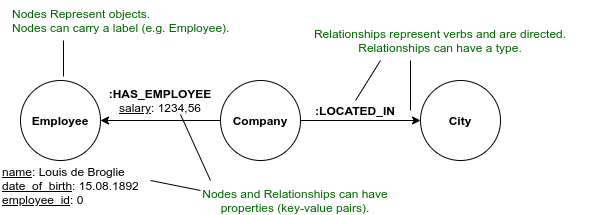
\includegraphics[keepaspectratio,width=0.6\textwidth]{img/03-preliminaries/property_graph_elements.png}
            \end{center}
            \caption{A schematic visualization of the property graph model.} 
            \label{propertygraph}
        \end{figure}

        
        Neo4j is a graph database employing the property graph model~\cite{robinson2015graph}.
        The logical operators of this model are described in~\autocite{Holsch2016Algeb}. 
        The \textit{get\_nodes}-operator returns all nodes of the graph.
        This means that however the nodes are stored, the whole file (portion) needs to be scanned.
        Further the \textit{expand}-operator returns the incident edges of a node depending on the direction.
        Expand only considers a part of the set of all edges, so it does not do full scans but rather smaller reads.
        Finally the \textit{filter}-operand selects certain nodes or relationships based on properties, labels or relationship type.
        
        In the next section \ref{n4j} we are going to discuss how Neo4J implements the property graph model, with our focus on the structure of the graph and the low level storage scheme.

    \subsection{Example: Neo4J}\label{n4j}
        Neo4J is a native graph database using the property graph model.
        The source code of the community edition is available at GitHub~\autocite{GitHubneo4j}.
        We look at some implementation details of the storage and buffer manager, as well as the record structure.
        We are not going to take properties, relationship types, labels and concepts related to those into account.
        
        \subsubsection*{High-level Architecture}
        \begin{figure}[htp]
            \begin{center}
                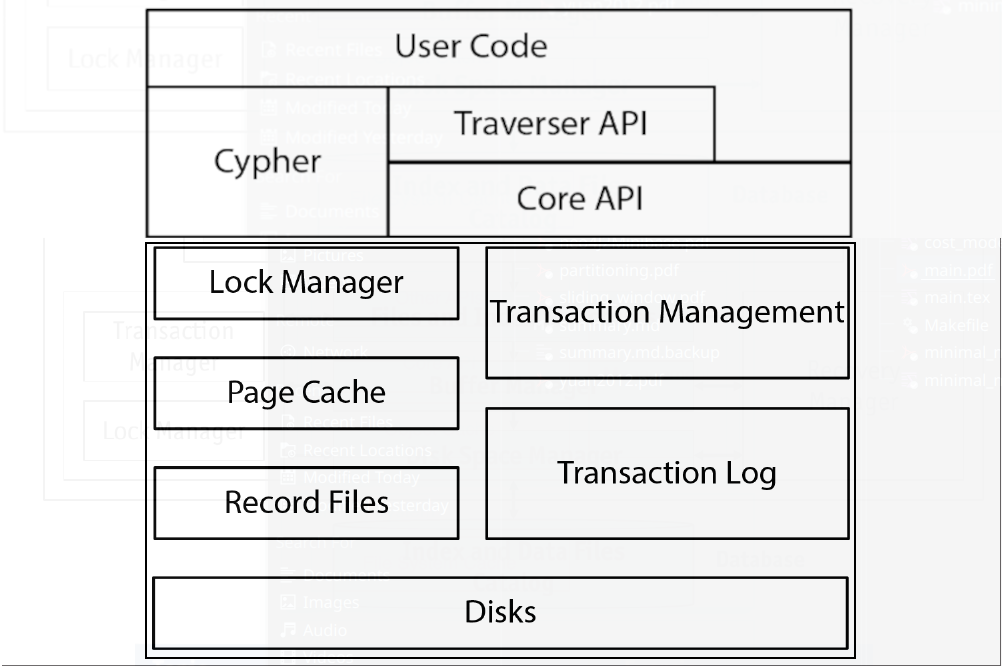
\includegraphics[keepaspectratio,width=0.25\textwidth]{img/03-preliminaries/N4J_HLA_Emil.png}
            \end{center}
            \caption{The high level architecture of Neo4J~\autocite{robinson2015graph}.} 
            \label{N4J_HLA_Emil}
        \end{figure}
        
        To get an overview of the architecture let us consider figure~\ref{N4J_HLA_Emil}.
        This description was outlined by the co-founder of Neo4J Emil Effrem, the chief science officer Jim Webber and Ian Robinson who was an engineer at that time at Neo4J in their book on graph databases~\autocite{robinson2015graph}.
        Here we can see that the architectural schema outlined in \ref{db-arch} and especially \ref{dbms_arch} was not quite applied.
        
        Still the components are very similar:
        The ''Page Cache`` is equivalent to the buffer manager, the record files are what is managed by the disk space manager, mechanisms to deal with free slots~\autocite{neo4jidgenerator} and (de-)allocations~\autocite{neo4jio} are also part of the software stack, as are the record formats~\autocite{neo4jrecordstorage} and indexes, corresponding to the access layer. 
        The corresponding components are just put together in a slightly different manner. 
        
        \begin{figure}[htp]
            \begin{center}
                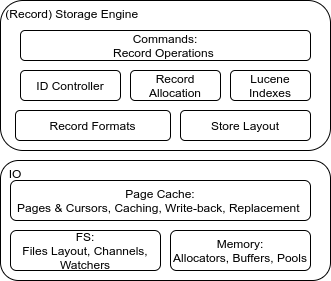
\includegraphics[keepaspectratio,width=0.5\textwidth,height=0.3\textheight]{img/03-preliminaries/N4J_Storage.png}
            \end{center}
            \caption{A visualization of the broad the storage and memory organization of Neo4J.} \label{N4J_Storage}
        \end{figure}
        
        The detailed composition is shown in ~\ref{N4J_Storage}.
        The IO package contains the page cache, which is basically the buffer manager.
        It also contains facilities to create, grow and shrink files using the \mintinline{java}{java.nio} library and wrappers arround platform dependent allocation facilities.
        Thus the (de-)allocation part of the disk space manager resides in the IO package, too.
        The record storage engine defines the record format and the file layout, as well as means to create and maintain indices, thus it is similar to the access layer. 
        It also handles the management of free slots something usually done by the disk space manager.
        To summarize: The buffer manager and the access layer correspond closely to these two packages, while the disk space manager is distributed mainly over these two packages.        

        \subsubsection*{Record and File Structures}
        Neo4J uses several different record types. They can be split broadly in the following categories:
        \begin{itemize}
         \item Variable size records: Strings, Arrays
         \item Fixed size records:
         \begin{itemize}
          \item Graph structure related records: Nodes, relationships, relationship groups
          \item Properties, labels, relationship types
         \end{itemize}
        \end{itemize}
        
        Each record type is stored in an own file per database in the database management system.
        An additional system database keeps track of the existence and metadata of the other ones storing user data.
        This is visualized in~\ref{n4j-disk}.
        \begin{figure}[htp]
            \begin{center}
                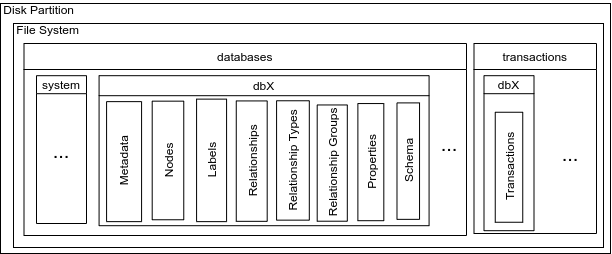
\includegraphics[keepaspectratio,height=0.4\textheight,width=0.7\textwidth]{img/03-preliminaries/N4J_disk_view.png}
            \end{center}
            \caption{A visualization of how the files are arranged of Neo4J.}
            \label{n4j-disk}
        \end{figure}
        
        The records are ordered simply by their insertion order, i.e. the files storing the records are heap files.
        While variable length records store strings and arrays, labels for example store a pointer to the actual string of the label to be fixed size and thus efficiently retreived.
        The same is true for relationship types and property keys and values that are stings or arrays.
        This is done to avoid duplications of strings e.g. of each label.
        As mentioned before for the sake of succintness we are just going to elaborate on the elements that represent the graph structure. 
        Only one thing is to be mentioned: 
        Properties are stored as a linked list for each nodes and relationships.
        
        \subsection*{Nodes}
            \begin{figure}[htp]
                \begin{center}
                    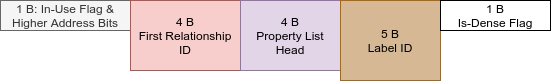
\includegraphics[keepaspectratio,height=0.4\textheight,width=0.7\textwidth]{img/03-preliminaries/node_record.png}
                \end{center}
                \caption{A visualization of the record structure of a node record~\autocite{neo4jNodeRecordFormat}.}
                \label{node-record-format}
            \end{figure}
            The record format of nodes consist of a 15 byte structure.
            The IDs of nodes are stored implicitly as their address.
            If a node has ID 100 we know that its record starts at offset $15 \text{ Bytes} \cdot 100 = 1500$ from the beginning of the file.
            The struct of a record looks like this:
            \begin{enumerate}
                \item Byte 1: One bit for the in-use flag. 
                The additional bits are used to compress the node struct by using the other 7 bits to store the most significant bits of the first relationship ID and the first property ID 
                \item Bytes 2 --- 5: The next 4 Bytes represent the relationship ID of the head in the linked list of relationships of the considered node.
                \item Bytes 6 --- 9: Again 4 bytes encode the property ID 0of the head in the linked list of properties of the node.
                \item Bytes 10 --- 14: This 5 byte section points to the labels of this node.
                \item Byte 15: The last byte stores if the node is dense, i.e.\ has an aweful lot of relationships, such that it needs special treatment in order to remain efficient to traverse over.
                That is a relationships are grouped by type and direction for this node.
            \end{enumerate}
            
            To summarize: The records on disk are stored as in the enumeration above and as shown in \ref{node-record-format}. 
            In the database all IDs get mapped to longs and their respective space is larger than the space representable by 35 bit --- what is perfectly fine.
            
            On disk 4 byte integers are used to store the 32 lowest bits of the respective addresses and the higher bits are stored in the first byte that also carries the in-use bit.
        
        \subsubsection*{Relationships}
            \begin{figure}[htp]
                \begin{center}
                    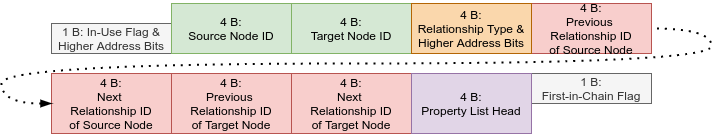
\includegraphics[keepaspectratio,height=0.9\textheight,width=0.9\textwidth]{img/03-preliminaries/relationship_record.png}
                \end{center}
                \caption{A visualization of the record structure of a relationship in Neo4J.}
                \label{rel_record}
            \end{figure}
                
            Relationship records are stored with implicit IDs too. 
            Their fixed size records contain 34 bytes.
            Besides an in-use flag, the source and target node IDs, and the relationship type, the record also contains two doubly linked list: 
            One for the incident edegs of the first node and one for the incident edges of the second node.
            Next a link to the head of the linked list of properties for this relationship is stored.
            Finally, the last byte contains a marker if this relationship is the first element in the incidence list of one of the nodes.
            
            \begin{enumerate}
                \item Byte 1: In-use bit, first node high order bits (3 bits), first property high order bits (4 bits)
                \item Bytes 2 --- 5: first node ID 
                \item Bytes 6 --- 9: second node ID 
                \item Bytes 10 --- 13: relationship type (16 bit), second node high order bits (3 bits), relationship previous and next ID higher bits for first and second node ($4 \cdot 3 = 12$ bits), one unused bit.
                \item Bytes 14 --- 17: previous relationship ID for first node
                \item Bytes 18 --- 21: next relationship ID for first node
                \item Bytes 22 --- 25: previous relationship ID for second node
                \item Bytes 26 --- 29: next relationship ID for second node
                \item Bytes 30 --- 33: link to the first property of the relationship
                \item Bytes 34: A marker if this relation is the first element in the relationship linked list of one of the nodes stored in the lowest two bits of the byte. 
                The other 6 bits are unused.
            \end{enumerate}
            
            \begin{figure}[htp]
                \begin{center}
                    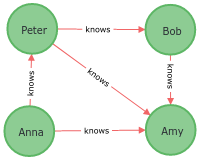
\includegraphics[keepaspectratio,height=0.4\textheight,width=0.4\textwidth]{img/03-preliminaries/graph.png}
                \end{center}
                \caption{An example graph.}
                \label{n4j-ex-gr}
            \end{figure}
            
            The relationship structure is a key element of the layout and reveals the actual data type that the database is using:
            Nodes and relationships are both stored once only (i.e. nothing is duplicated).
            Without taking the fields into account, this is an unordered edge list.
            When taking the linked lists of relationships into account, it turns out that the underlying data structure is that of an indicence list, with a couple of additional properties.
            
            First, as already mentioned, the edges are not physically duplicated but only referenced. 
            The records are fixed sized, so addressing them is done by multiplying the index by the size of an entry, meaning one does not need to store primary keys explicitly and adress translation can be done using a simple multiplication. 
            Theoretically one could align the record size to a power of two to turn the multiplication into a bit shift.
            Next, as doubly linked lists are used, the deletion of an edge is in $\mathcal{O}(1)$ if the ID is known.
            If this was not the case, the incidence list would need to be traversed in order to find the previous element.
            Also, the incidence list is stored in the relationships.
            Thus in order to traverse from one node's incidence list to another, there is no need to load the node record itself.
            It suffices to just dereference the next element in the incidence list stored by the relationships, along with storing the ID of the edge that started the traversal.
            This makes the assumption, that the doubly linked incidence lists is circular, i.e. the head's pervious element is the tail and reciprocally.

            To conclude this example, we briefly visualize the just described storage schema. 
            The high-level graph is shown in \ref{n4j-ex-gr}.
            It contains four nodes and five edges.
            The underlying instantiated data structures are shown in \ref{n4j-ex}.
            The light red arcs represent edges, the light green circles nodes.
            The colored boxes on the edges and nodes represent the data structures.
            The brighter red edges represent the doubly linked incidence lists.
            Notice, that the heads and tails of the doubly linked incidence lists are marked by ''X`` to avoid to draw additional edges.
            The brighter green arrows represent the source and target nodes, as stored by the edges. \\
            \vfill
            \begin{figure}[htp]
                \begin{center}
                    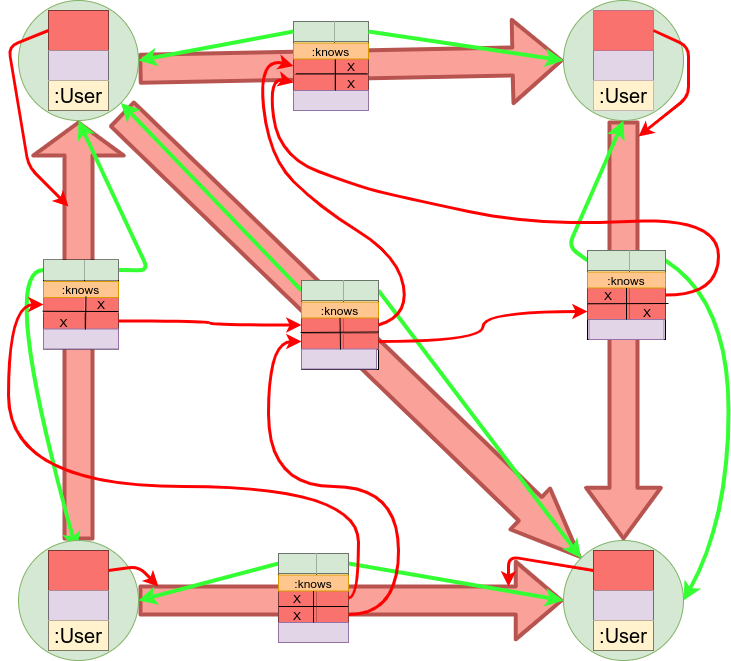
\includegraphics[keepaspectratio,height=\textheight,width=\textwidth]{img/03-preliminaries/example_structs.png}
                \end{center}
                \caption{Visualization of the data structures, as initialized by the example graph shown in \ref{n4j-ex-gr}.}
                \label{n4j-ex}
            \end{figure}
            \vfill
